\documentclass[12pt]{article}
\usepackage{hyperref}
\usepackage{microtype}
\usepackage{multirow}
\usepackage{amsmath}
\usepackage{amssymb}
\usepackage{graphicx}
\usepackage[left=2.5cm,top=2.5cm,right=2.5cm,bottom=2.5cm]{geometry}
\usepackage{natbib}

\hypersetup{
    colorlinks=true,
    linkcolor=blue,
    urlcolor=blue,
    breaklinks=true
}
\usepackage{xurl}



\title{Bridging the Gap: Analyzing Auction Prices and Day-Ahead Market Discrepancies at the Swiss-German Electricity Border}
\author{Nicolas Greber \and Vansh Khanna \and Massimo Nardo }
\date{December 10, 2024}

\begin{document}
\sloppy
\maketitle

\begin{abstract}

This short paper analyzes cross-border electricity pricing between Switzerland and Germany, focusing on mispricing and market inefficiencies. Using hourly data from 2019–2023, we evaluate pricing deviations through statistical tests. Results confirm mean-reverting deviations, supporting the convergence hypothesis, but reveal significant temporal dependencies and abrupt volatility increases during the 2022–2023 energy crisis.
\end{abstract}




\newpage
% Table of Contents


\newpage

\section{Introduction}

Switzerland's electricity markets are not part of the European Market Coupling system. As a result, electricity trading across the borders between Switzerland and Germany occurs explicitly rather than through automatic coupling mechanisms. This analysis investigates whether the border prices for importing and exporting electricity between Switzerland and Germany reflect the market price differences in both regions. Additionally, we aim to identify patterns in pricing errors, should the border prices fail to perfectly represent these differences.

\subsection{Background}

Electricity is a unique commodity. One distinguishing feature is that demand and supply must match perfectly at any given moment. Furthermore, electricity flows through a grid with finite capacity, imposing additional constraints. To ensure the balance between demand and supply, electricity is traded at different times before delivery in different markets. Although there is over-the-counter trading, a large part of the trading takes place on centralized exchanges such as EPEX and EEX. 

\begin{itemize}
    \item \textit{Futures Market:} Traded on exchanges such as EEX, this market allows electricity to be bought and sold for delivery periods ranging from days to six years in advance.
    \item \textit{Day-Ahead Market:} The market for securing hourly electricity delivery for the following day. The intermediary is EPEX. Most European countries participate in coupled day-ahead markets, which automatically trade electricity across borders. Switzerland, however, is not part of this coupling system. Instead, it has its own day-ahead market.
    \item \textit{Intraday Market:} Used for same-day electricity trading. EPEX facilitates this market. 
    \item \textit{Ancillary Services Market:} Ensures grid stability through balancing services. Transmission system operators (TSOs) instruct suppliers or demanders to adjust production or consumption, maintaining supply-demand balance even on a second-by-second level. This market includes primary, secondary, and tertiary control reserves, differentiated by response time and cost.
\end{itemize}

Switzerland's electricity supply companies, holding monopolies over households with regulated pricing, can purchase electricity on the Swiss day-ahead market or import it from neighboring countries like Germany, incurring additional import costs. Limited border capacity is auctioned by the Joint Allocation Office (JAO) on yearly, monthly, and daily bases, with revenues shared between the respective TSOs. Similarly, German producers can sell electricity domestically or export it to Switzerland, factoring in export costs.

This setup results in an arbitrage argument. Price differences between the Swiss and German day-ahead markets should align with the import and export costs at the border, ensuring buyers and exporters are indifferent between market options. Specifically:
\begin{itemize}
    \item If the Swiss electricity price exceeds the German day-ahead price:
    \begin{itemize}
        \item Buyers in Switzerland should be indifferent between purchasing electricity domestically or importing from Germany, considering import costs.
        \item Exporters in Germany should be indifferent between selling to the German market or exporting to Switzerland, accounting for export costs.
    \end{itemize}
    \item If the German electricity price exceeds the Swiss price:
    \begin{itemize}
        \item Buyers in Germany should be indifferent between purchasing electricity domestically or importing from Switzerland, including import costs.
        \item Exporters in Switzerland should be indifferent between selling domestically or exporting to Germany, factoring in export costs.
    \end{itemize}
\end{itemize}


\subsection{Hypotheses}

Based on this market setup, we formulate the following hypotheses:

\begin{itemize}
    \item \textit{The Convergence Hypothesis:} The price difference between Germany and Switzerland, adjusted for border costs in both directions, equals zero. This equilibrium arises from arbitrage opportunities and the absence of transaction costs in JAO auctions.
    \item \textit{The Independence Hypothesis:} Any observed pricing errors are uncorrelated over time, indicating no systematic patterns in their occurrence.
    \item \textit{The Volatility Growth Hypothesis:} Pricing accuracy has deteriorated as solar capacity expansion creates more unpredictable supply-demand patterns.
\end{itemize}
To illustrate the increase in solar PV in Switzerland, see Figure \ref{fig:pv_increase}.

\begin{figure}[ht]
    \centering
    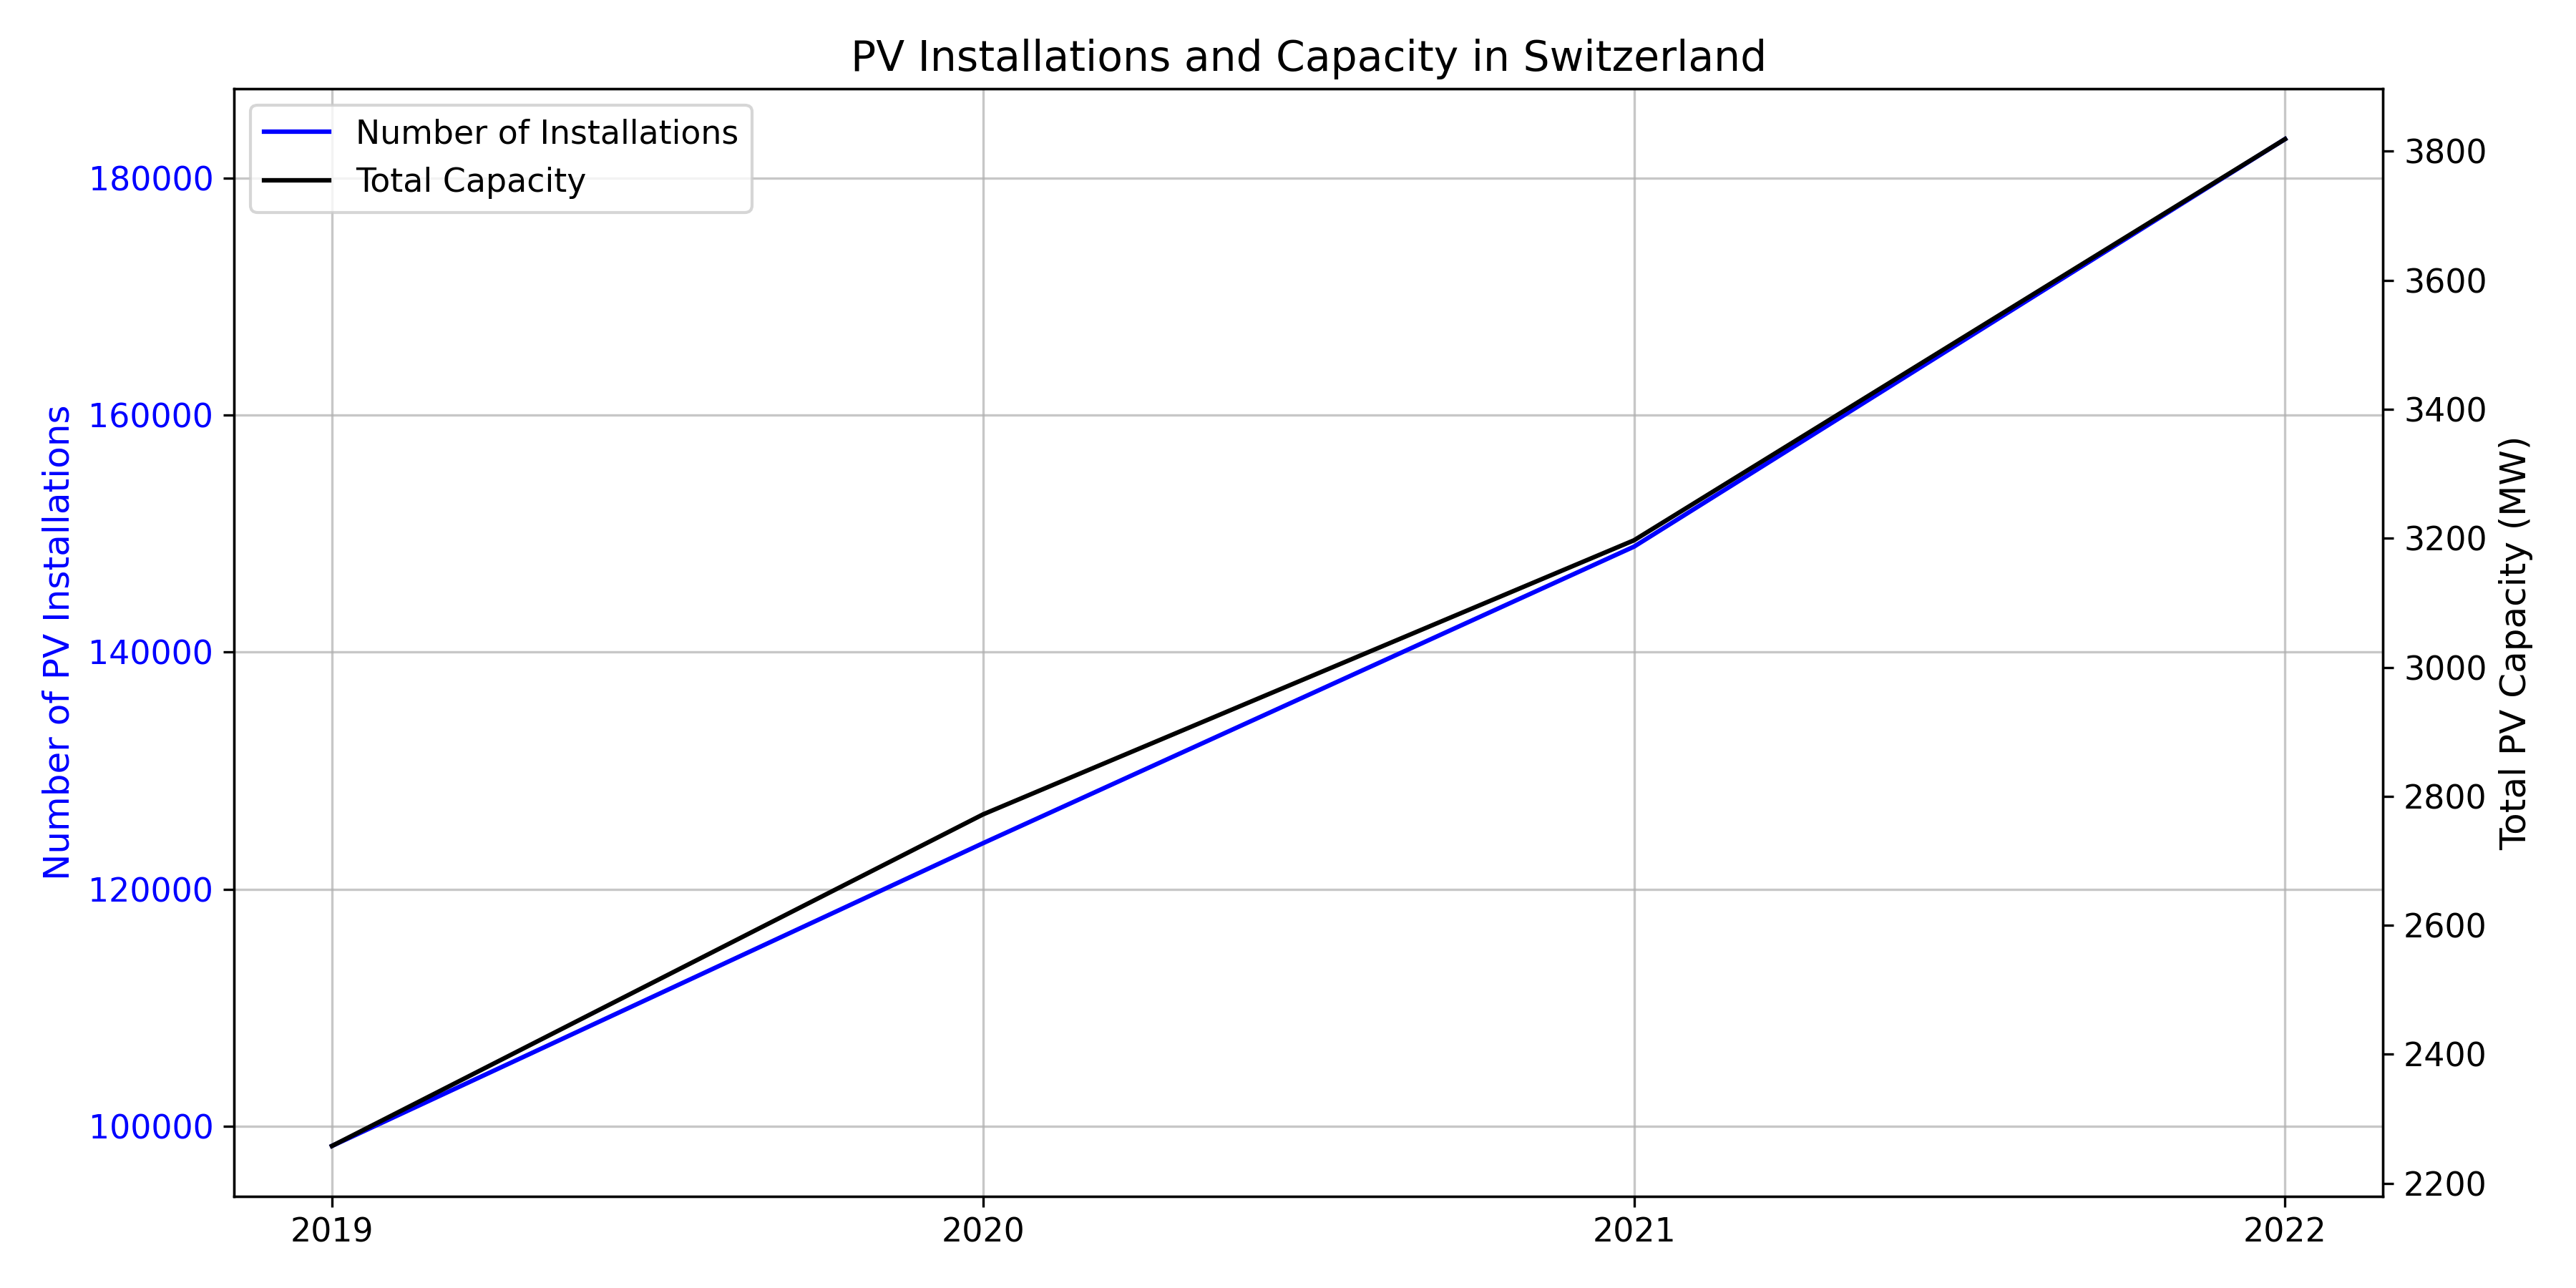
\includegraphics[width=0.75\textwidth]{figures/pv_installations_switzerland.png}
    \caption{Trends in the number of photovoltaic (PV) installations and total PV capacity in Switzerland from 2019 to 2022. The blue line (left axis) represents the cumulative number of PV installations, while the black line (right axis) indicates the total installed PV capacity in megawatts (MW). The steady increase in both metrics reflects the growing adoption of solar energy in Switzerland.}
    \label{fig:pv_increase}
\end{figure}

This paper analyzes the cross-border electricity prices between Switzerland and Germany, focusing on potential mispricing in these interconnected markets. While previous studies, such as \cite{keles2020cross} have examined the broader influences of neighboring countries on Swiss electricity prices using econometric models and equilibrium simulations, our research takes a different approach. 



\section{Data and Methodology}

This analysis explores the relationship between cross-border electricity auction prices and day-ahead market prices in Switzerland (CH) and Germany-Luxembourg (DE-LU). According to efficient market theory, the price difference between markets should align with transaction costs. Deviations from this relationship may indicate inefficiencies or barriers within the market.

\subsection{Data}

We utilize data from multiple sources, covering the period from 2019 to 2023. These include day-ahead market prices, auction prices for cross-border capacities, and photovoltaic (PV) capacity data. The data preparation and sources are detailed below:

\subsubsection*{Day-Ahead Market Prices}

Day-ahead prices for Switzerland, Germany-Luxembourg and Germany-Austria-Luxembourg were downloaded from the Entso-E Transparency platform.\footnote{\href{https://transparency.entsoe.eu/}{Entso-E Transparency Platform}} The dataset spans 2016 to 2023. However, a significant market change occurred on October 1, 2018, when Austria was excluded from the Germany-Luxembourg day-ahead market region. For consistency in our analysis, we restrict the dataset to the period 2019 to 2023.

Day-ahead markets trade electricity in hourly intervals for the following day. Settlement for the Swiss day-ahead market occurs at 11:00 CET, while for most European countries, including Germany, it happens at 12:00 CET.\footnote{\href{https://www.epexspot.com/en/basicspowermarket\#day-ahead-and-intraday-the-backbone-of-the-european-spot-market}{EPEX Spot: Day-ahead and Intraday Market Overview}} Bids consist of size and price, forming the supply and demand curves. The market-clearing price is determined by the intersection of these curves, using a uniform pricing mechanism.

\subsubsection*{Cross-Border Auction Prices}

Cross-border auction prices were obtained from the Joint Allocation Office (JAO). These auctions allocate limited transmission capacity for electricity between countries. For Switzerland, daily capacities are auctioned for each hour of the next day. The auctions take place the day before delivery, with the final bids accepted at 09:30 CET.\footnote{For detailed rules, refer to \href{https://www.jao.eu/resource-center/auction-rules}{JAO Auction Rules \citep{AllocationRules2023}} and select ``CH Auction Rules 2023.'' For auction results, visit \href{https://www.jao.eu/auctions\#/}{Auction Results}.} Each auctioned megawatt of capacity represents the right to transport one megawatt-hour of electricity across the border during a specific hour.

The auction price data covers the period from 2019 to 2023. We downloaded this data using the JAO API.\footnote{The download process is documented in the README file of the project's GitHub repository.}

\subsubsection*{Photovoltaic Data}

Photovoltaic (PV) capacity data was sourced from the Swiss Federal Office of Energy (SFOE).\footnote{\href{https://www.bfe.admin.ch/bfe/de/home/versorgung/statistik-und-geodaten/monitoring-energiestrategie-2050.exturl.html/aHR0cHM6Ly9wdWJkYi5iZmUuYWRtaW4uY2gvZGUvcHVibGljYX/Rpb24vZG93bmxvYWQvMTAzMjI=.html}{Monitoring Report by the Swiss Federal Office of Energy}} This dataset includes yearly data on installed PV capacity and the total number of PV installations. Since the data contains only a few points, we manually converted it from Excel to a CSV format for analysis.

\subsection{Variables}

The analysis uses hourly data from 2016 to 2023. Key variables are summarized below:
\begin{table}[ht]
    \footnotesize
    \centering
    \begin{tabular}{|l|p{6cm}|l|}
        \hline
        \textit{Variable} & \textit{Description} & \textit{Unit} \\ \hline
        \( p_t^{CH} \) & Day-ahead price in Switzerland & EUR/MWh \\ \hline
        \( p_t^{DE} \) & Day-ahead price in Germany-Austria-Luxembourg (Includes prices for the market region \( DE-AT-LU \) before October 1, 2018, and \( DE-LU \) thereafter) & EUR/MWh \\ \hline
        \( p_t^{CH \rightarrow DE} \) & JAO Auction Price: Switzerland to Germany & EUR/MWh \\ \hline
        \( p_t^{DE\rightarrow CH} \) & JAO Auction Price: Germany to Swit-zerland & EUR/MWh \\ \hline
        Installed Capacity & Yearly installed PV capacity in Switzerland & MW \\ \hline
        Number of PV Units & Total number of installed photovoltaic units & Count \\ \hline
    \end{tabular}
    \caption{Key variables used in the analysis.}
\end{table}

The error term, denoted as $\delta_t$ is defined as
\begin{equation}
    \delta_t = p_t^{DE} + p_t^{DE \rightarrow CH} - p_t^{CH} - p_t^{CH \rightarrow DE}.
\end{equation}
This term measures deviations between the Swiss-German price spread and the auction price, potentially reflecting inefficiencies in cross-border pricing. \newline
The normalized error term $\hat{\delta}_t$ is 
\begin{equation}
    \hat{\delta}_t = \frac{\delta_t}{(p_t^{CH} + p_t^{DE})/2}.
\end{equation}
Normalized by the average price of the two markets to account for different price levels of the day-ahead prices over the time. 

\subsection{Statistical Tests}

To evaluate market efficiency and identify potential inefficiencies in cross-border electricity pricing, we apply a series of statistical tests to the error term $\delta_t$ and its normalized counterpart $\hat{\delta}_t$. These tests assess whether pricing deviations are temporary, systematic, or indicative of broader structural issues.

\subsubsection*{Stationarity Test: Augmented Dickey-Fuller (ADF)}

The first test examines whether the error term $\delta_t$ is stationary, which is a key property for market efficiency. A stationary series implies that deviations are temporary and mean-reverting, while non-stationarity indicates persistent pricing inefficiencies. We use the Augmented Dickey-Fuller (ADF) test to formally evaluate this property.

The hypotheses are as follows:
\begin{itemize}
    \item Null Hypothesis ($H_0$): $\delta_t$ has a unit root, indicating non-stationarity.
    \item Alternative Hypothesis ($H_1$): $\delta_t$ is stationary, suggesting mean-reverting deviations.
\end{itemize}

Stationarity in $\delta_t$ supports the notion that arbitrage opportunities are temporary and corrected over time. In contrast, non-stationarity may indicate barriers to arbitrage or structural inefficiencies in the cross-border electricity market.

\subsubsection*{Mean Test with HAC Adjustment}

To investigate whether the average error term deviates systematically from zero, we conduct a mean test on $\delta_t$. Under efficient market conditions, pricing deviations should balance out over time, resulting in a mean of zero.

To ensure robust inference, the Newey-West Heteroskedasticity and Autocorrelation Consistent (HAC) estimator is applied, accounting for potential autocorrelation and heteroskedasticity in the time series.

The hypotheses for this test are:
\begin{itemize}
    \item Null Hypothesis ($H_0$): $\mathbb{E}[\delta_t] = 0$, implying no systematic mispricing.
    \item Alternative Hypothesis ($H_1$): $\mathbb{E}[\delta_t] \neq 0$, indicating persistent pricing discrepancies.
\end{itemize}

A non-zero mean in $\delta_t$ suggests inefficiencies, where auction prices fail to fully reflect the cost of cross-border electricity trade.

\subsubsection*{Autocorrelation Analysis}

The temporal dependencies in $\delta_t$ are analyzed using autocorrelation at lag 24 (one day).

The autocorrelation coefficient is defined as:
\begin{equation}
    \rho_{24} = \frac{\text{Cov}(\delta_t, \delta_{t-24})}{\text{Var}(\delta_t)}
\end{equation}

Temporal dependencies in $\delta_t$ could arise from systematic forecast errors or cyclical patterns, potentially revealing inefficiencies in cross-border price adjustments.

\subsubsection*{Variance Trend Analysis}

To investigate whether the variability of pricing deviations changes systematically over time, we analyze the normalized error term $\hat{\delta}_t$. This approach evaluates whether variance exhibits a temporal trend, potentially reflecting shifts in market dynamics or structural inefficiencies. 

The rolling variance of $\hat{\delta}_t$ is computed over a fixed time window (e.g., 30 days) to capture short-term variability. A linear regression model is then fitted to detect systematic trends:
\begin{equation}
    \sigma_t(\hat{\delta}_t) = \alpha + \beta t + \epsilon_t,
\end{equation}
where $\beta$ represents the temporal trend in variance. 

The hypotheses for this analysis are:
\begin{itemize}
    \item Null Hypothesis ($H_0$): $\beta = 0$, indicating no systematic trend in variance.
    \item Alternative Hypothesis ($H_1$): $\beta \neq 0$, suggesting a statistically significant trend in variance over time.
\end{itemize}

An increasing trend ($\beta > 0$) may suggest growing uncertainty or inefficiencies in cross-border pricing, possibly driven by structural changes such as increased renewable energy penetration. Conversely, a decreasing trend ($\beta < 0$) could indicate improving market alignment or enhanced pricing mechanisms.

This test complements the variance ratio analysis by capturing gradual changes in variability, providing additional insights into temporal dynamics in pricing inefficiencies.

\subsubsection*{Variance Ratio Test}
To assess changes in variability, we apply a variance ratio test comparing the variance of $\hat{\delta}_t$ between two distinct time periods. 

The variance ratio, which follows an F-distribution, is defined as:
\begin{equation}
    F = \frac{\text{Var}(\hat{\delta}_t \text{ (later period)})}{\text{Var}(\hat{\delta}_t \text{ (earlier period)})} \sim F(n_1 - 1, n_2 - 1),
\end{equation}
where $n_1$ and $n_2$ are the number of observations in the later and earlier periods, respectively.

The hypotheses are:
\begin{itemize}
    \item $H_0$: The variances in the two periods are equal
    \item $H_1$: The variances in the two periods are not equal
\end{itemize}
A significant result ($p < 0.05$) suggests that variability in cross-border pricing deviations has changed between the two periods.



% Results
\section{Results}

\subsection{Observable Dynamics}

The first part of the analysis examines the relationship between auction prices for electricity transport between Switzerland (CH) and Germany (DE). We hypothesize that if the auction price for transporting electricity from CH to DE is positive, the auction price for the reverse direction (DE to CH) should be zero, and vice versa.

\begin{figure}[h!]
    \centering
    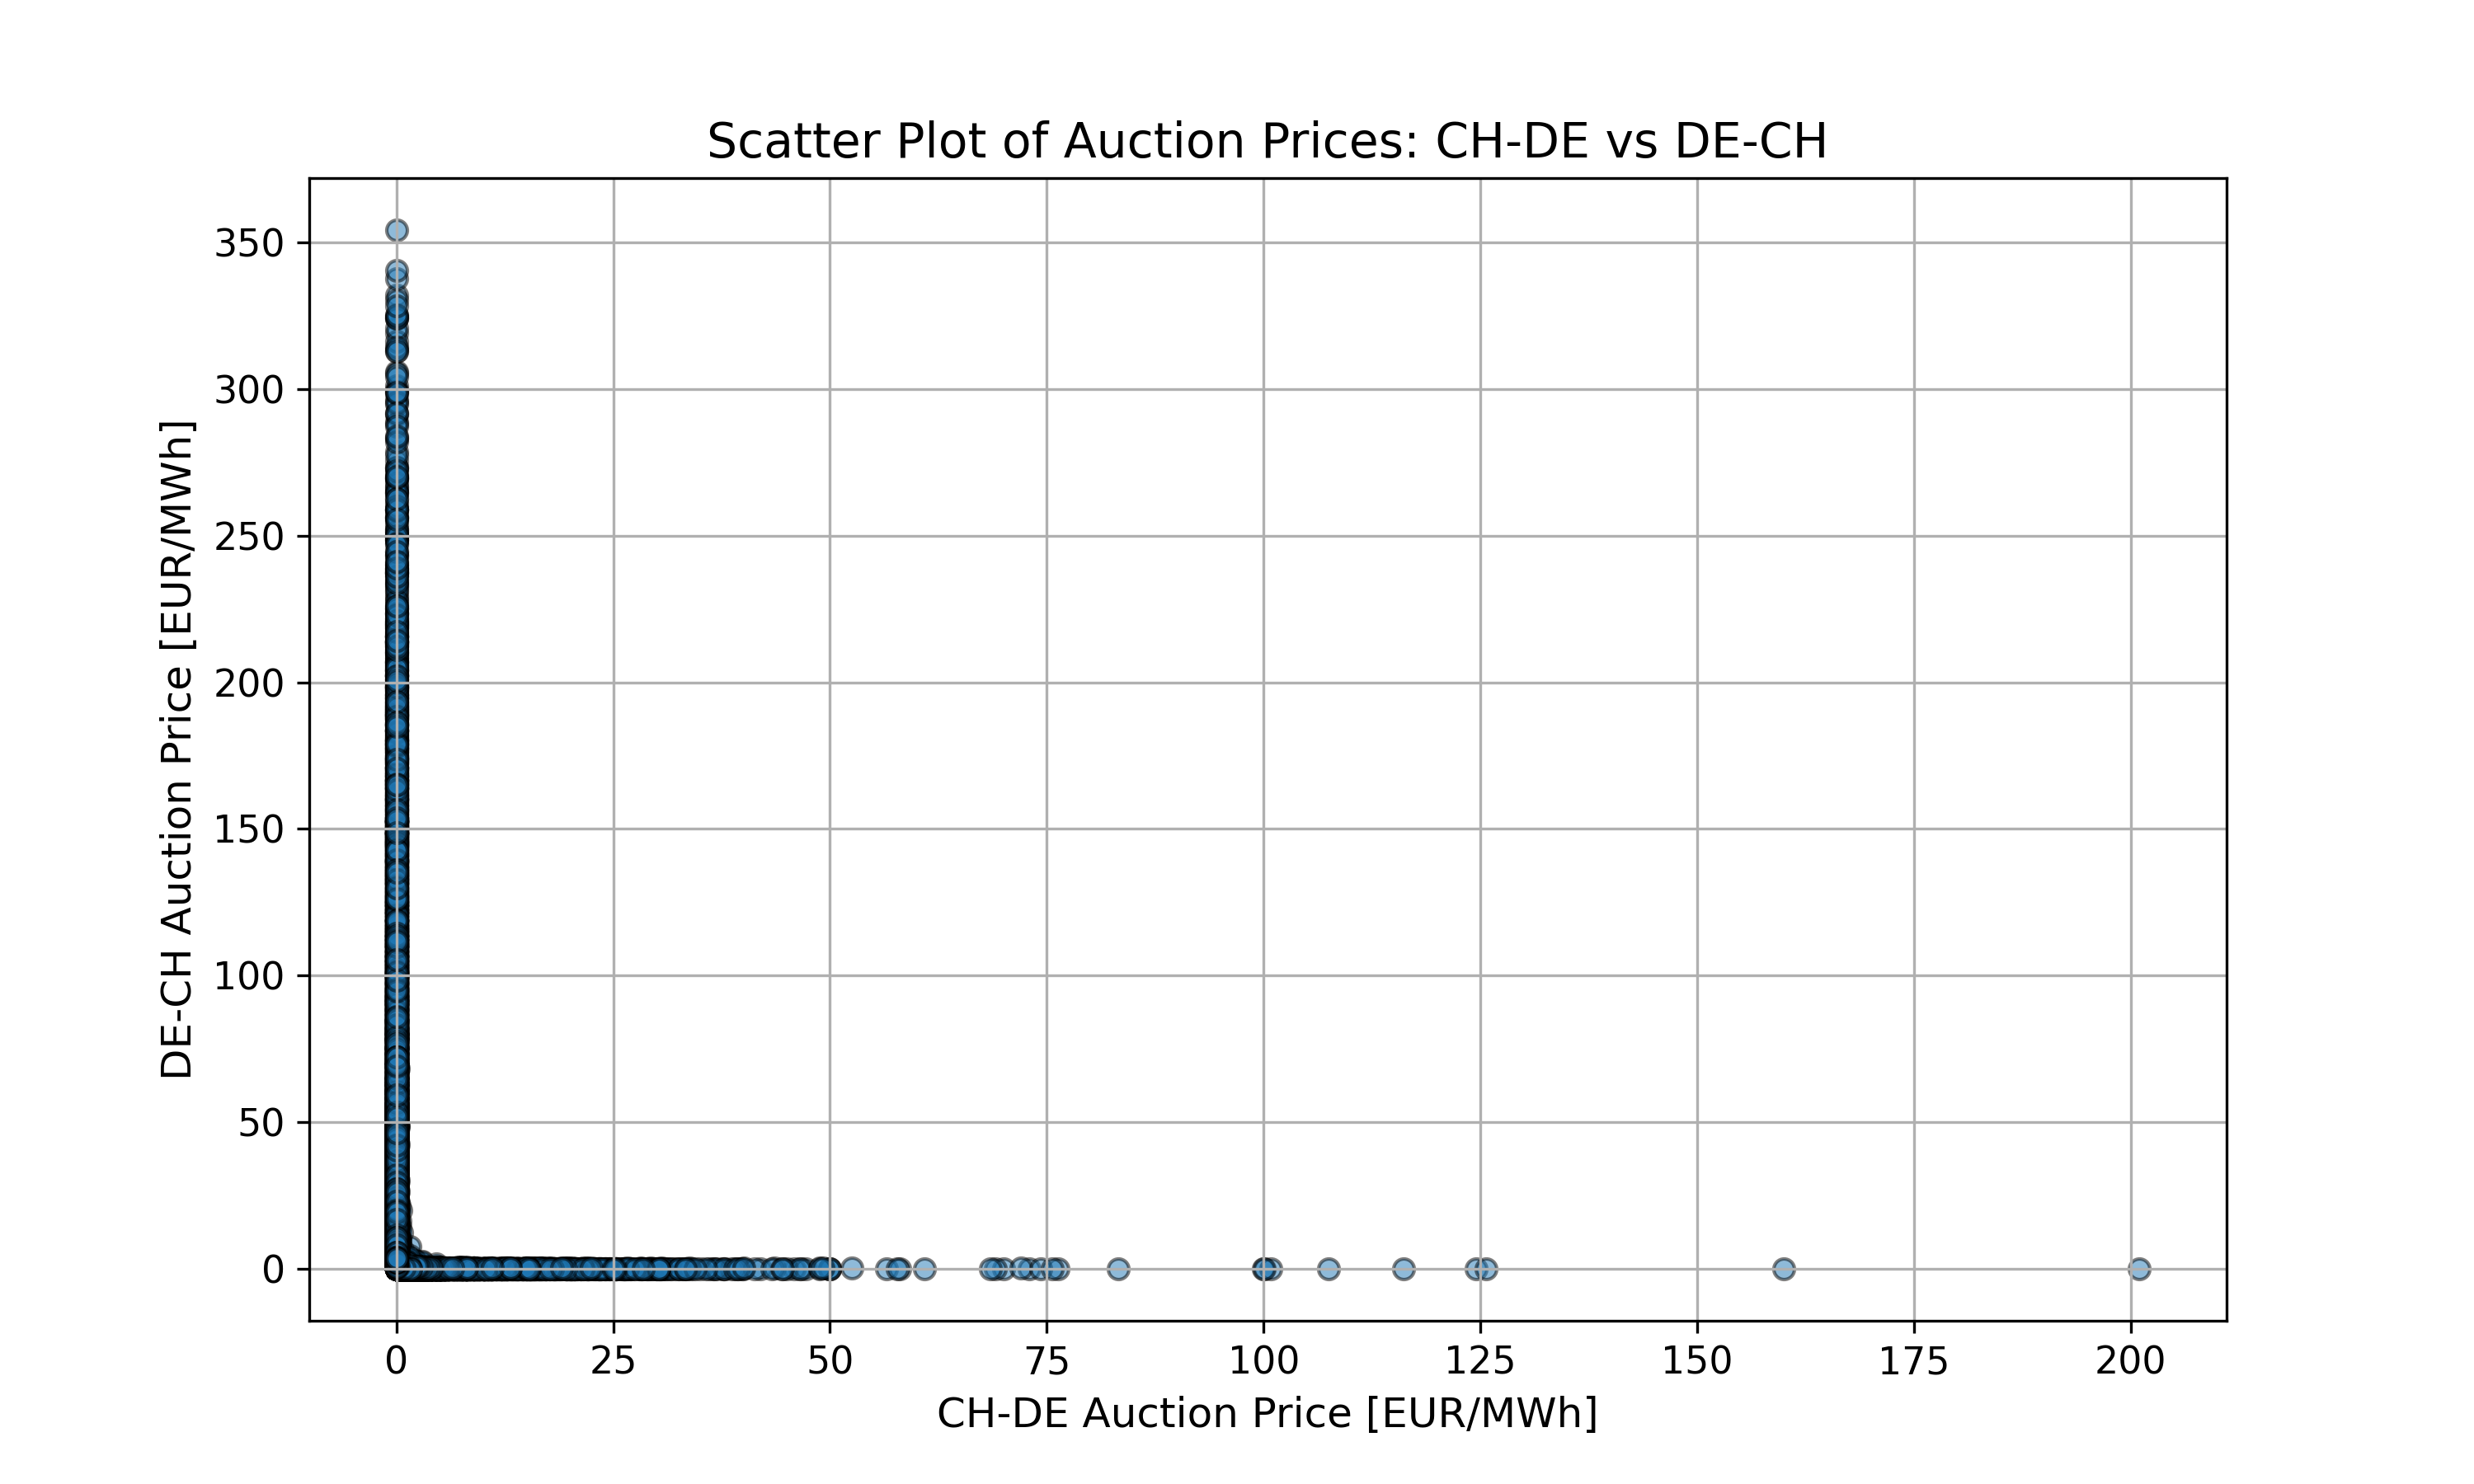
\includegraphics[width=0.75\textwidth]{figures/scatter_plot_ch_de_vs_de_ch_auction_prices.png}
    \caption{Scatter plot of auction prices for CH$\rightarrow$DE versus DE$\rightarrow$CH, illustrating that auction prices are set in one direction only, confirming (almost) mutual exclusivity of positive auction prices.}
    \label{fig:scatter_ch_de_auction}
\end{figure}

\noindent
Figure \ref{fig:scatter_ch_de_auction} confirms this hypothesis. Observations cluster around $(0, y)$ with $y \geq 0$ or $(x, 0)$ with $x \geq 0$, indicating that auction prices are set exclusively in one direction. This behavior reflects the intended functionality of the auction mechanism, ensuring no overlap in pricing between the two directions.

Next, we analyze the weekly averages of the adjusted day-ahead price difference $\delta_t$.

\begin{figure}[ht]
    \centering
    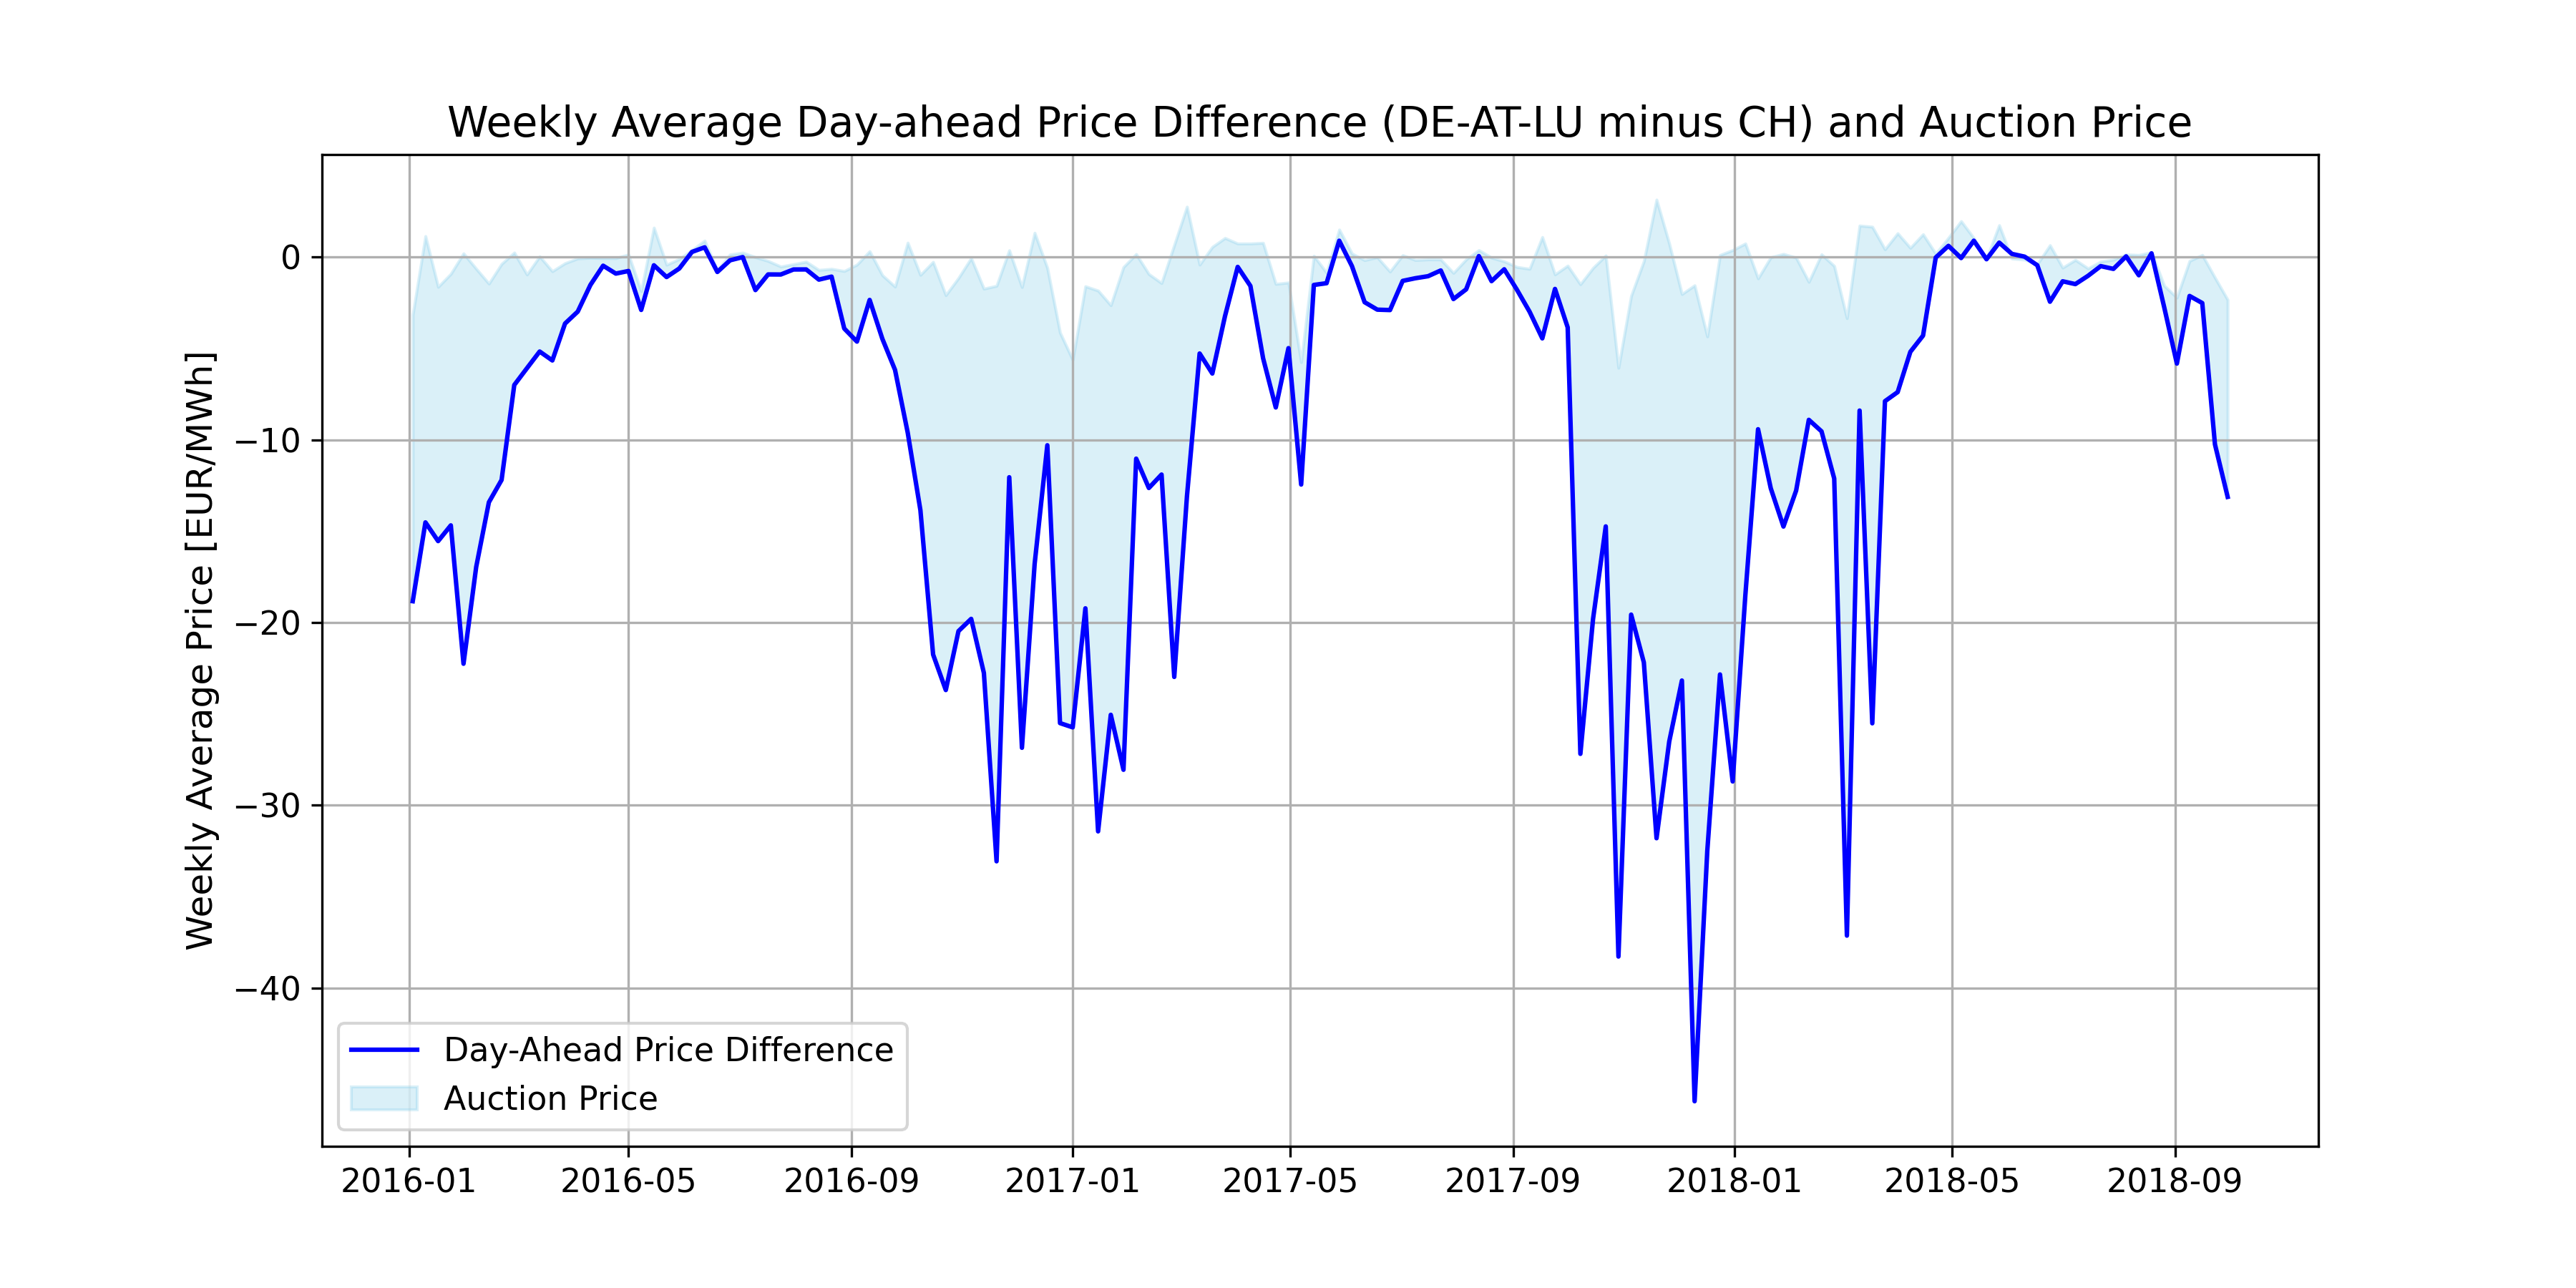
\includegraphics[width=0.75\textwidth]{figures/weekly_average_day_ahead_price_diff_de-lu-at_ch.png}
    \caption{Weekly average day-ahead price difference (DE-AT-LU minus CH) and auction prices. The shaded area represents the adjusted price difference, accounting for auction prices.}
    \label{fig:weekly_de_at_lu_ch}
\end{figure}

\begin{figure}[ht]
    \centering
    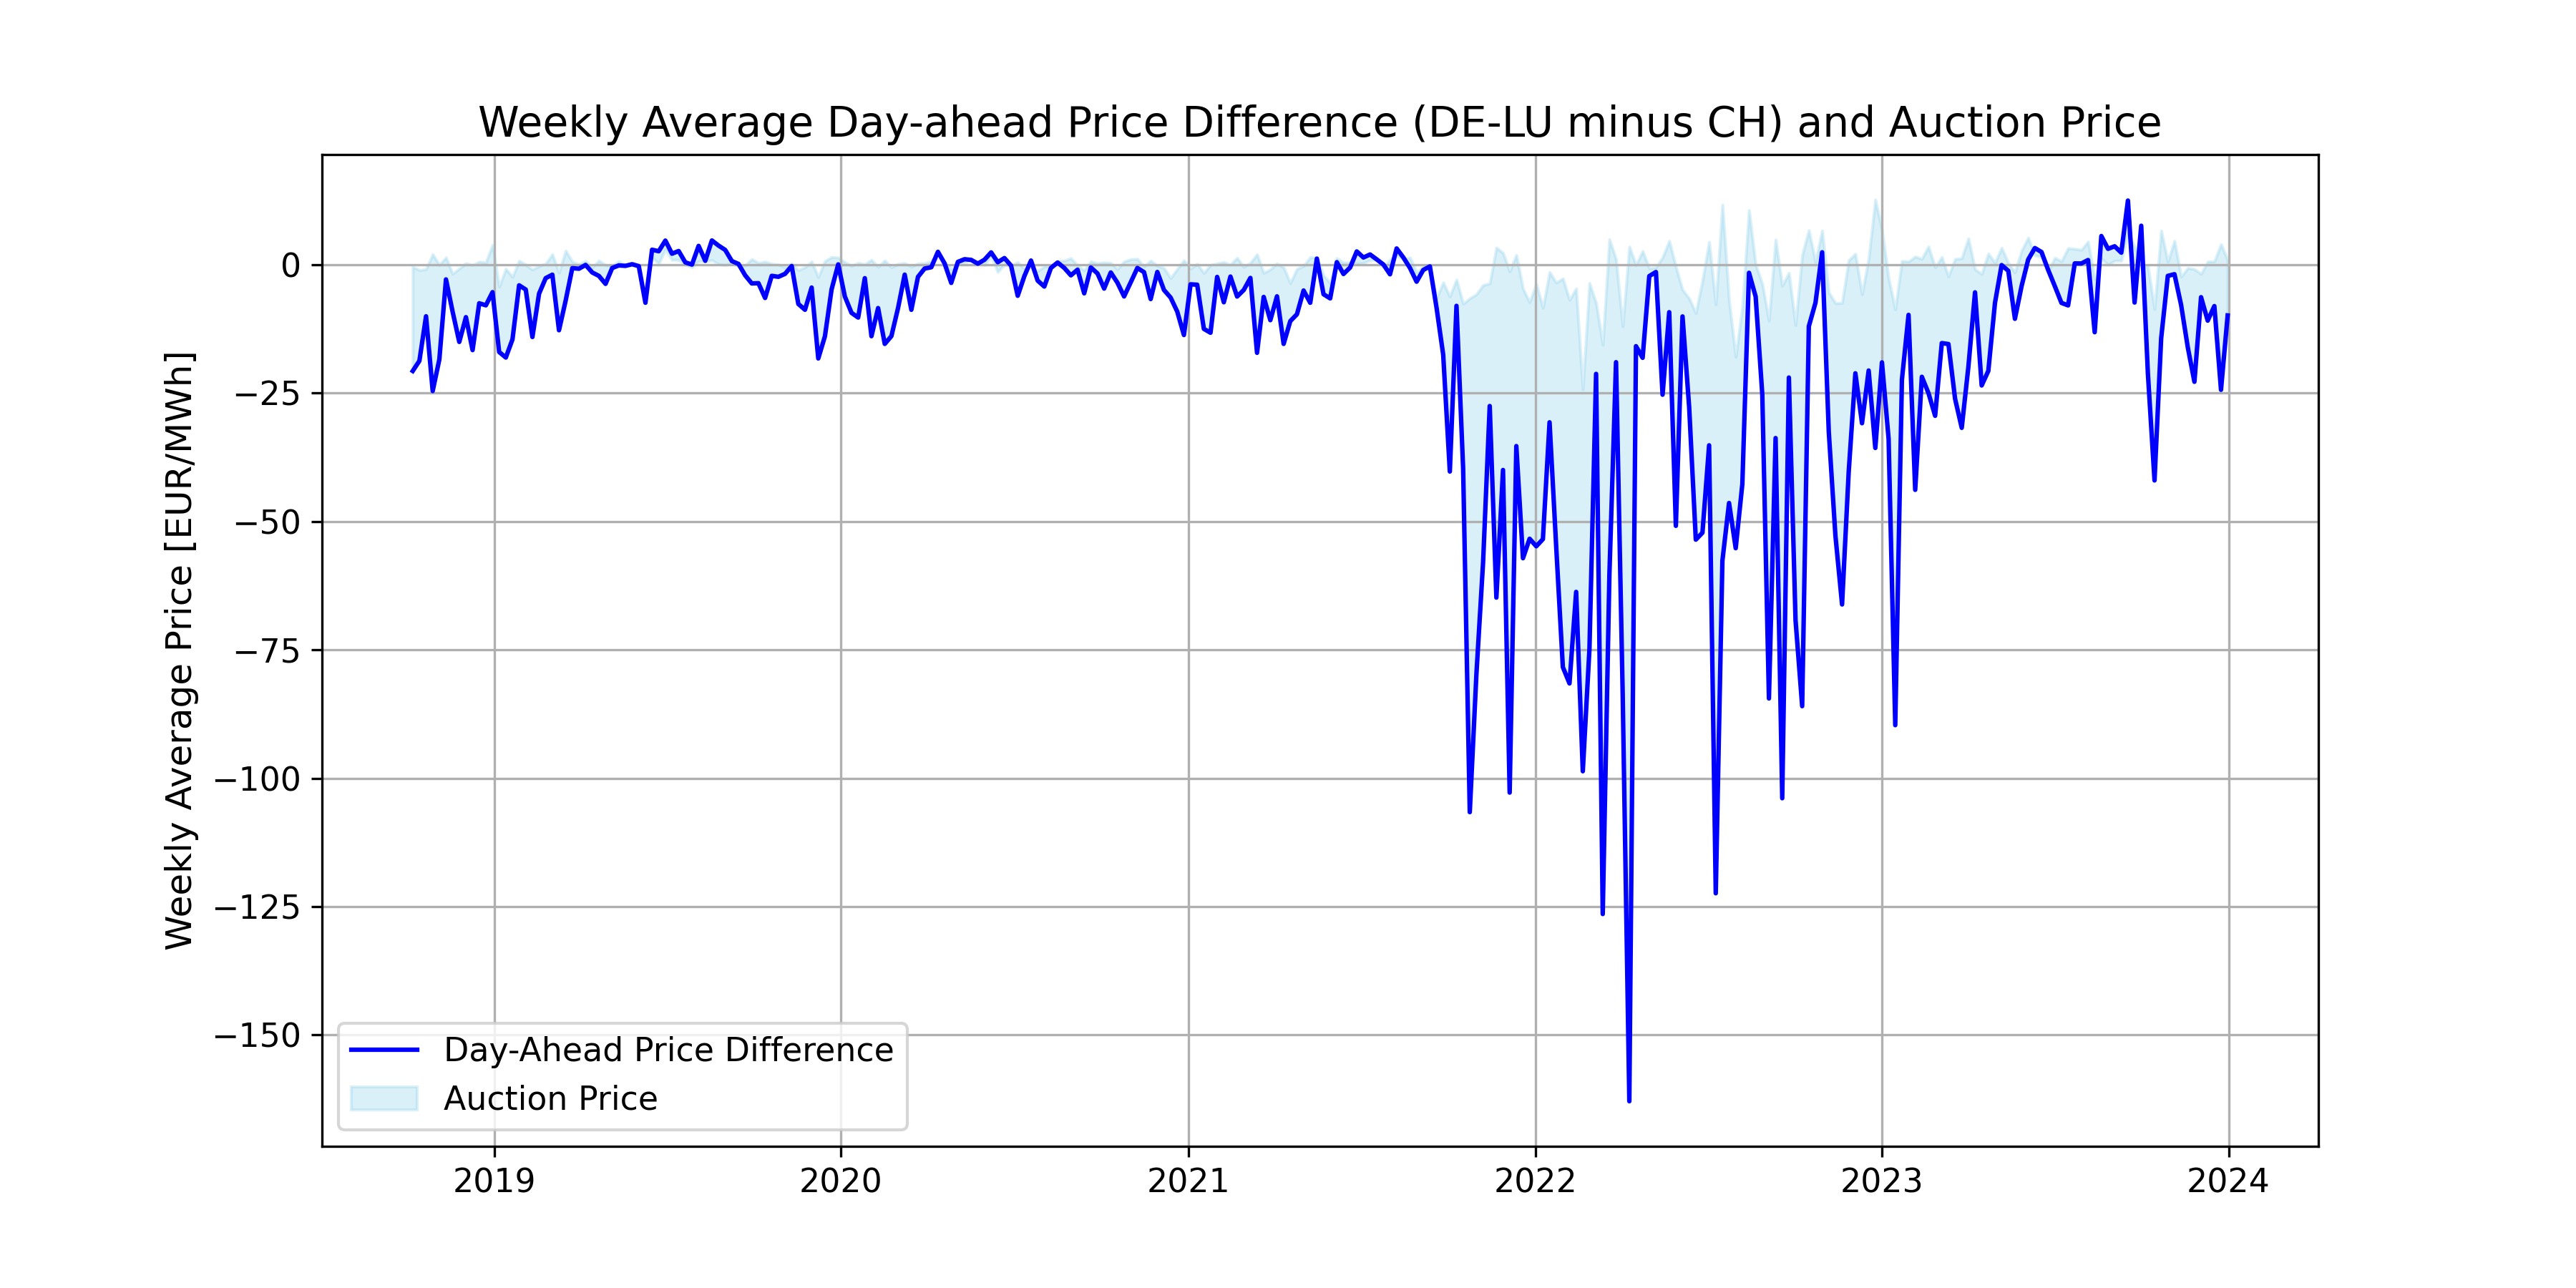
\includegraphics[width=0.75\textwidth]{figures/weekly_average_day_ahead_price_diff_de-lu_ch.png}
    \caption{Weekly average day-ahead price difference (DE-LU minus CH) and auction prices. The shaded area reflects the adjusted price difference, showing alignment with zero under efficient market conditions.}
    \label{fig:weekly_de_lu_ch}
\end{figure}

\noindent
Figures \ref{fig:weekly_de_at_lu_ch} and \ref{fig:weekly_de_lu_ch} present the weekly average day-ahead price differences for the DE-AT-LU and DE-LU market regions relative to CH, respectively. 

The blue line illustrates the unadjusted price difference, showing that CH prices are generally higher than DE prices, with a pronounced seasonal pattern. Price differences are larger during winter months and narrower in summer, likely reflecting variations in demand and energy mix.

The shaded areas incorporate auction prices to represent the adjusted price differences. Under efficient market conditions, these adjusted differences should converge to zero, indicating that weekly averages of auction prices fully account for disparities in weekly averages of day-ahead market prices.

The shaded areas in both figures align closely with zero for most periods, suggesting that auction prices effectively offset day-ahead market price differences.

Deviations from zero, particularly during the energy crisis from late 2021 to 2022, highlight potential inefficiencies or market disruptions caused by external factors such as supply shortages. Note the differing y-axis scales in Figures \ref{fig:weekly_de_at_lu_ch} and \ref{fig:weekly_de_lu_ch}.

\noindent
These results suggest that the auction mechanism functions as intended under normal market conditions in weekly averages, effectively compensating for cross-border price differences.


Next we examine the statistical properties of the $\delta_t$. The analysis uses hourly data from 2019 onward (DE-LU), ensuring that the change in the German pricing market region in 2018 does not influence the results.

Figure \ref{fig:error_series} provides a comprehensive view of the error term over time and its rolling statistics. The top plot shows the hourly error term $\delta_t$, while the bottom plot presents the rolling mean and standard deviation, to identify trends in central tendency and variability.

\begin{figure}[ht]
    \centering
    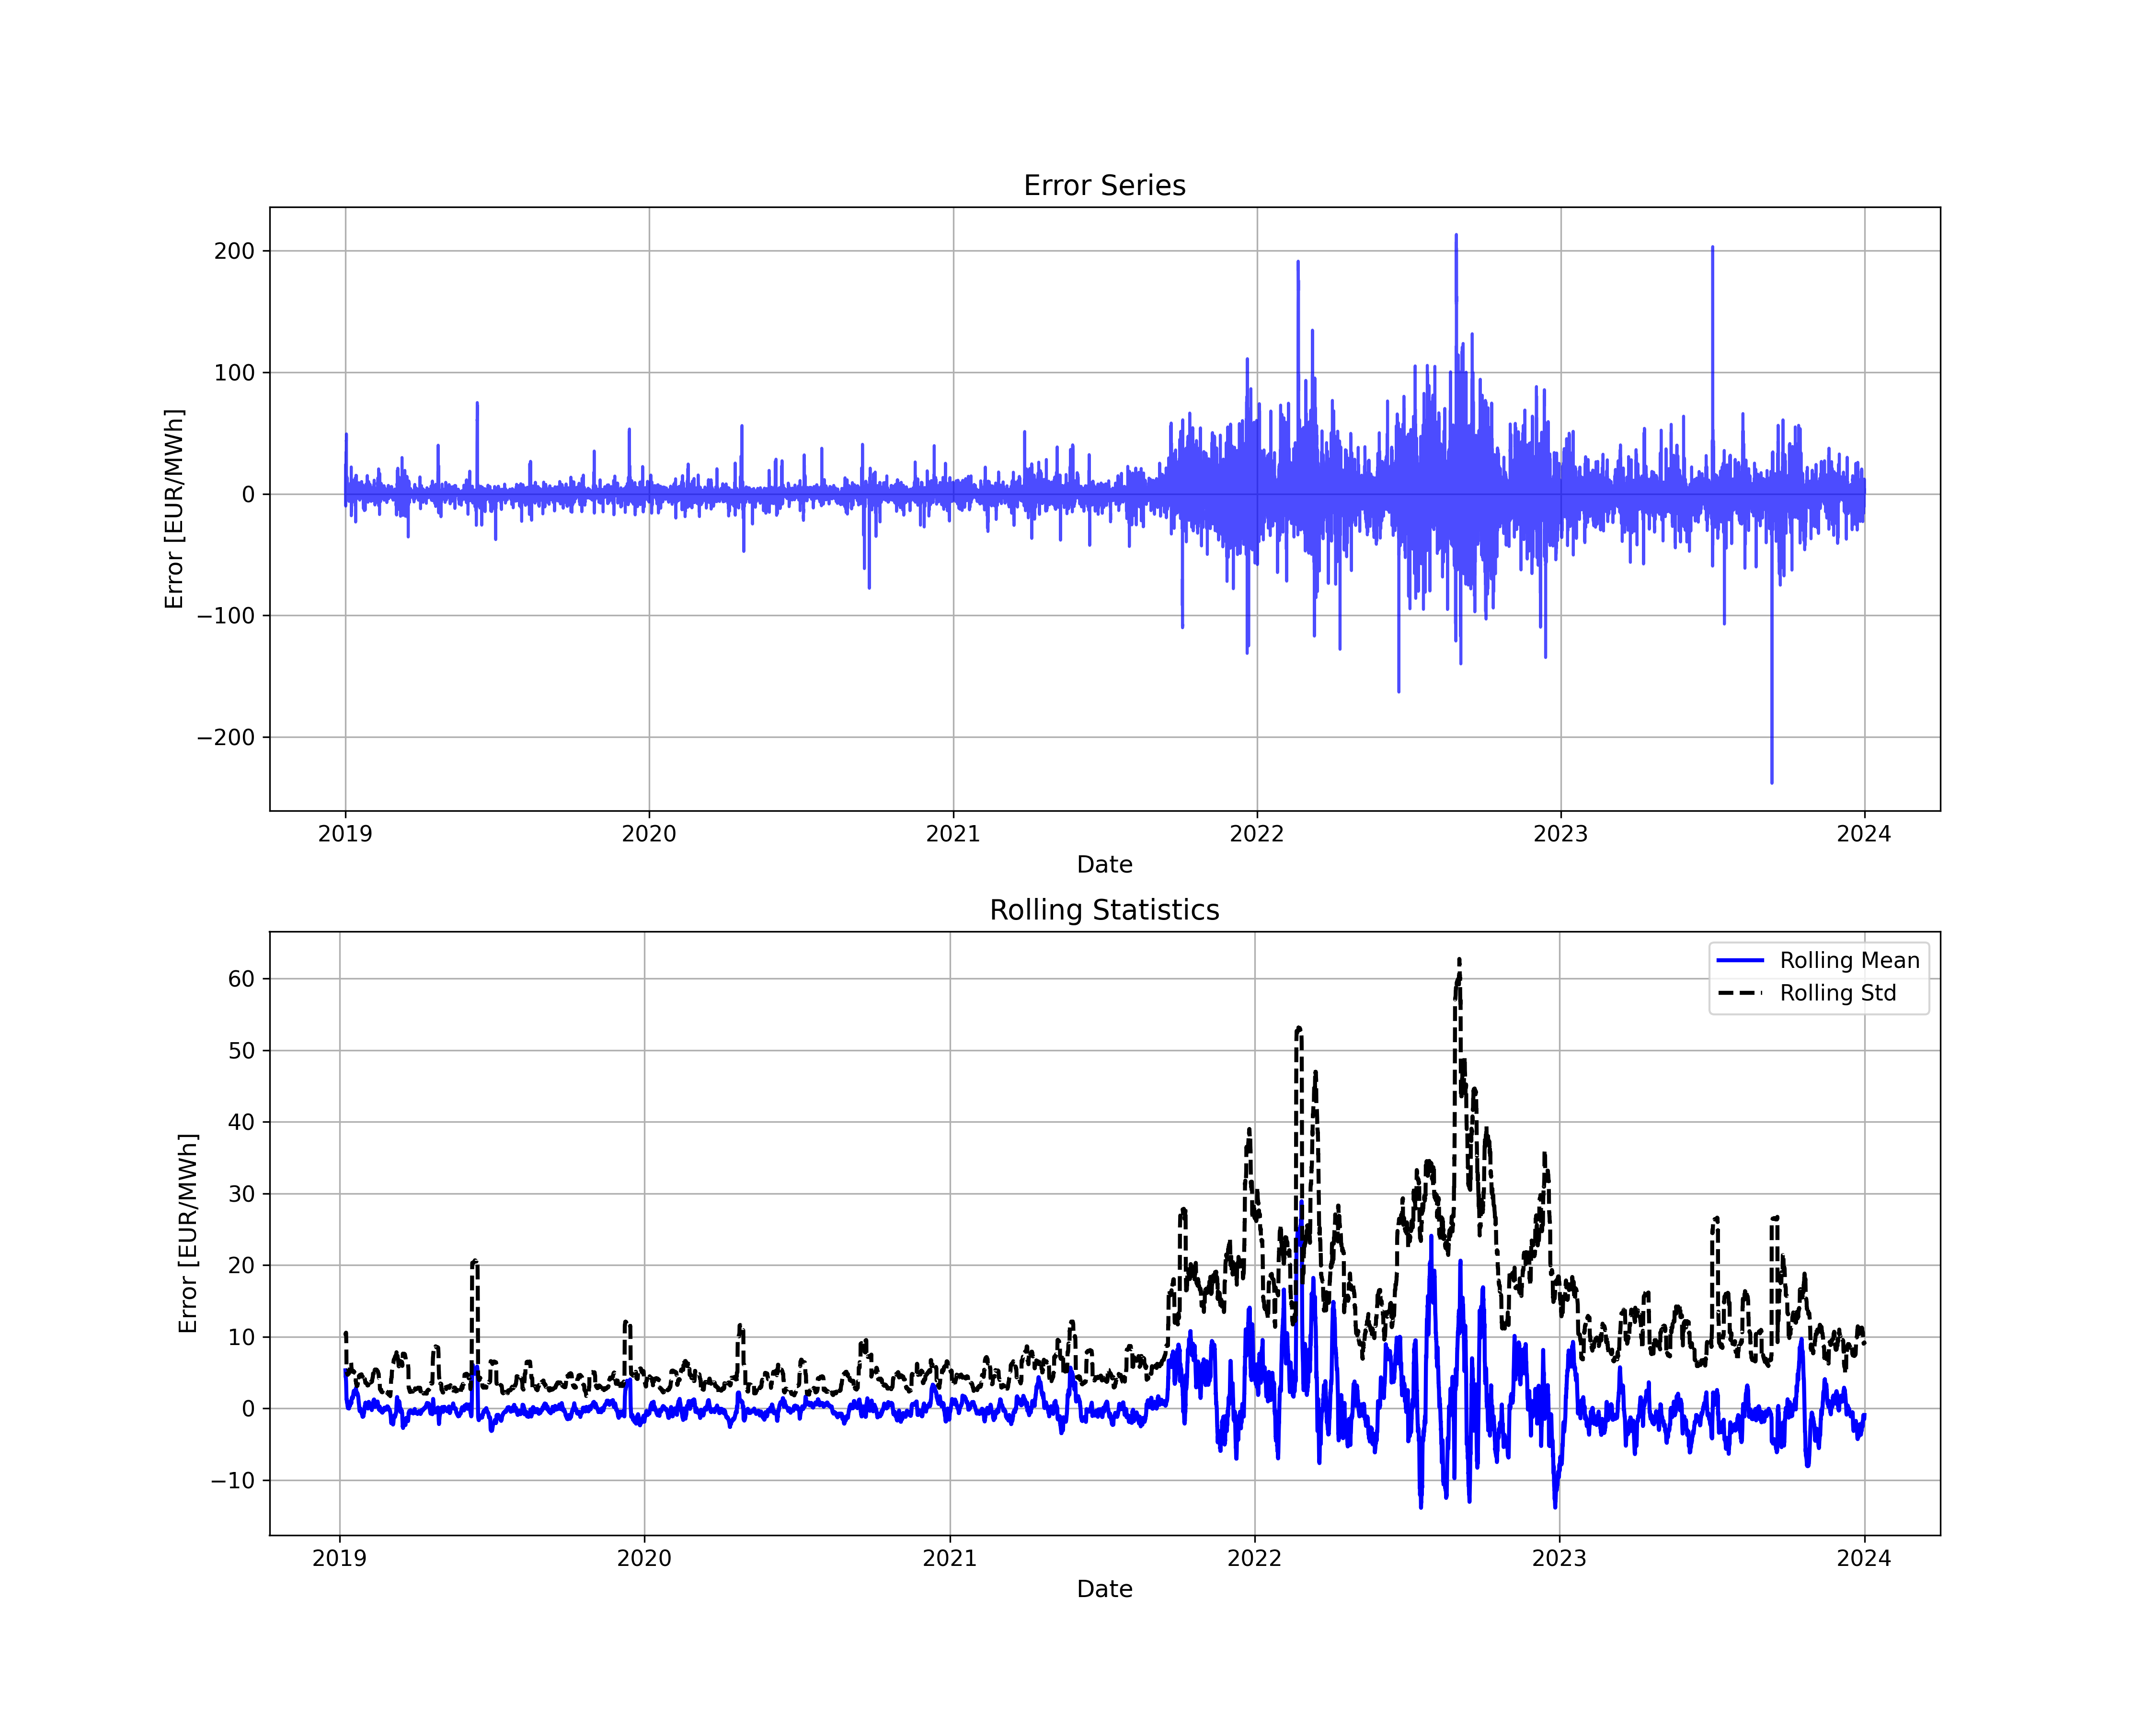
\includegraphics[width=0.75\textwidth]{figures/error_series.png}
    \caption{Hourly error series (top plot) and rolling statistics (bottom plot). The error series illustrates deviations between auction prices and day-ahead price differences, while the rolling mean and standard deviation capture trends in central tendency and variability.}
    \label{fig:error_series}
\end{figure}

The error term $\delta_t$, depicted in the top plot, remains mostly centered around zero throughout the observation period, suggesting a mean-reverting process consistent with efficient market behavior. This behavior indicates that deviations in auction prices from day-ahead price differences are typically corrected over time. However, starting in 2022, significant spikes and dips in the error term emerge, highlighting periods of increased volatility.

The bottom plot further analyzes these dynamics through the rolling mean and standard deviation. The rolling mean consistently hovers near zero, reinforcing the absence of a persistent trend in the error term over the observed period. This stability supports the hypothesis that the cross-border auction mechanism generally aligns well with day-ahead price differences under normal conditions. In contrast, the rolling standard deviation exhibits a sharp increase during 2022 and 2023, indicating a notable rise in volatility in $\delta_t$.



\subsection{Statistical Tests}

The results of the statistical tests are presented in Table \ref{tab:test_results}, with detailed interpretations provided below. The tests evaluate the convergence, independence, and volatility growth hypotheses based on the statistical properties of the error term.

\begin{table}[ht]
   \footnotesize
   \centering
   \caption{Summary of Statistical Test Results}
   \label{tab:test_results}
   \begin{tabular}{lrrc}
       \hline
       \textit{Test} & \textit{Value} & \textit{P-value} & \textit{Inference} \\
       \hline
       ADF Test & -26.112 & 0.000 & Stationary \\
       HAC Test & 2.175 & 0.030 & Mean deviation \\
       Autocorrelation (Lag 24) & 0.021 & 0.000 & Serial correlation \\
       Variance Trend & 1.00e-5 & 0.959 & No trend \\
       Variance Ratio & 2.685 & 0.000 & Variance increase \\
       \hline
   \end{tabular}
\end{table}

\textit{The Augmented Dickey-Fuller (ADF)} test confirms that the error term is stationary, as indicated by the strongly negative ADF statistic and the highly significant p-value ($p < 0.001$). This result supports the convergence hypothesis, suggesting that deviations from the expected price difference are temporary and mean-reverting.

The \textit{HAC-adjusted t-test} reveals a small but statistically significant mean deviation of the error term from zero ($p < 0.05$). This result implies that while deviations are generally temporary, there may be systematic inefficiencies or biases in the auction mechanism that warrant further exploration.

Significant \textit{autocorrelation is observed at lag 24}, with an autocorrelation coefficient (ACF) of 0.0206 and a highly significant p-value ($p < 0.001$). This finding rejects the independence hypothesis, indicating potential temporal patterns or dependencies in pricing errors, particularly over daily cycles.

The \textit{variance trend test} detects no significant increase in the variance of the normalized error term over time. The negligible slope and high p-value ($p = 0.9585$) suggest that linear volatility growth is not evident across the studied period.

The \textit{variance ratio test} identifies a significant increase in variance between the earlier and later periods, with a variance ratio of 2.6850 and a highly significant p-value ($p < 0.001$). Whether the increase in variance of the standardized error $\hat{\delta}_t$ is due to an increase in PV or due to the market stress is not clear with the tests done. 

\subsection{Statistical Tests by Year}

To further investigate the temporal dynamics of pricing deviations, the statistical tests were conducted for each year from 2019 to 2023. Table \ref{tab:yearly_test_results} summarizes the results for the Augmented Dickey-Fuller (ADF) test, HAC-adjusted t-test, and autocorrelation at lag 24.
\begin{table}[ht]
   \footnotesize
   \centering
   \caption{Statistical Test Results by Year}
   \label{tab:yearly_test_results}
   \begin{tabular}{l|rr|rr|rr}
       \hline
       \textit{Year} & \textit{ADF} & \textit{p-value} & \textit{HAC t-stat} & \textit{p-value} & \textit{Autocorr (Lag 24)} & \textit{p-value} \\
       \hline
       2019 & -17.470 & 0.000 & -0.295 & 0.768 & -0.048 & 0.000 \\
       2020 & -21.344 & 0.000 & -1.117 & 0.264 &  0.032 & 0.003 \\
       2021 & -13.774 & 0.000 &  2.903 & 0.004 &  0.026 & 0.015 \\
       2022 & -13.362 & 0.000 &  2.557 & 0.011 &  0.016 & 0.138 \\
       2023 & -15.799 & 0.000 & -2.341 & 0.019 &  0.017 & 0.121 \\
       \hline
   \end{tabular}
\end{table}


The \textit{ADF test} consistently indicates that the error term $\delta_t$ is stationary across all years, as evidenced by highly negative ADF statistics and p-values close to zero. This result supports the convergence hypothesis, implying that deviations in cross-border electricity pricing are mean-reverting regardless of the year. Even during volatile periods, such as 2022, the stationarity of the error term suggests that the market mechanism retains its ability to correct pricing discrepancies over time.

The \textit{HAC-adjusted t-test} reveals considerable variation in the statistical significance of the mean error term across years. For example:
\begin{itemize}
    \item In 2019 and 2020, the mean deviations are not statistically significant, with p-values well above $0.05$. These findings indicate that, under normal market conditions, the mean pricing error is negligible.
    \item In 2021, 2022 and 2023, the t-statistics indicate significant deviations from zero, suggesting potential inefficiencies.
\end{itemize}
The results for 2021 and 2022 align with the increased market volatility during the energy crisis, highlighting periods of stress in the cross-border electricity market.


The \textit{autocorrelation coefficient at lag $24$} shows varying significance across years:
\begin{itemize}
    \item In 2019 and 2020, significant autocorrelation is observed ($p = 0.0000$ and $p = 0.003$), indicating systematic dependencies in pricing errors over daily cycles. These dependencies may reflect structural inefficiencies or recurring forecast errors during these years.
    \item From 2021 onward, the autocorrelation becomes less significant, with p-values of $0.015$ in 2021 and above $0.1$ in 2022 and 2023. This reduction in significance suggests that, despite heightened volatility in 2022, pricing errors exhibit fewer systematic patterns, possibly due to improved forecasting or market adjustments.
\end{itemize}

\section{Discussion}

This study provides valuable insights into the dynamics of cross-border electricity pricing between Switzerland and Germany, analyzed through the convergence, independence, and volatility growth hypotheses. The findings confirm certain expected market behaviors while revealing inefficiencies and temporal variations that merit further investigation.

\subsection{Evaluation of Hypotheses}

\paragraph{Convergence Hypothesis}

The stationarity of the error term $\delta_t$, confirmed by the ADF test, strongly supports the convergence hypothesis. This result suggests that deviations from the expected price difference, adjusted for auction costs, are temporary and mean-reverting, even during volatile periods such as the 2022 energy crisis. The stationarity of $\delta_t$ underscores the robustness of the auction mechanism in aligning cross-border electricity prices under both normal and stressed market conditions.

However, the HAC-adjusted t-test identifies significant mean deviations from zero in specific years, particularly in 2021 and 2022. These deviations, though small in magnitude, are statistically significant, pointing to potential inefficiencies or market frictions. Such inefficiencies may stem from structural constraints, auction design limitations, or external factors, particularly during periods of heightened market stress.

\paragraph{Independence Hypothesis}

The independence hypothesis is challenged by the autocorrelation test results. Significant autocorrelation at lag 24 (representing daily cycles) is observed in the earlier years (2019–2020), indicating systematic temporal dependencies in pricing errors. These dependencies may reflect structural inefficiencies, recurring forecast errors, or operational constraints in the auction mechanism.

Interestingly, the significance of autocorrelation diminishes from 2021 onward, particularly during the 2022 energy crisis. This reduction may reflect improvements in market forecasting models, better integration of renewable energy forecasts, or adaptive market responses to evolving supply-demand dynamics. Nonetheless, the observed temporal patterns underscore the need for ongoing refinement of forecasting and operational practices.

\paragraph{Volatility Growth Hypothesis}

The results for the volatility growth hypothesis present a nuanced picture. The variance trend test finds no significant linear increase in the normalized error term's variance over time, suggesting that volatility growth is not a consistent trend across the study period. However, the variance ratio test reveals a marked increase in variance during the later years, particularly in 2022 and 2023, coinciding with the energy crisis.

This abrupt increase in variance raises questions about its underlying drivers. While the expansion of solar photovoltaic (PV) capacity may contribute to increased price volatility through more variable supply, the results also highlight the role of broader market stressors, such as geopolitical tensions and supply chain disruptions. Further research is required to disentangle these effects and better understand their contributions to market dynamics.

\subsection{Future Research Directions}

The results of this study highlight several avenues for further research:
\begin{itemize}
    \item \textbf{Geographic Comparisons:} Extending the analysis to other cross-border electricity markets, such as Switzerland-France or Switzerland-Italy, could provide comparative insights into regional differences and uncover common or unique patterns in pricing dynamics.
    \item \textbf{Long-Term Products:} Investigating the alignment of auction prices with longer-term products, such as yearly futures, would offer a broader perspective on price convergence and market efficiency over extended time horizons.
    \item \textbf{Renewable Integration:} A detailed analysis of the impact of renewable energy expansion, particularly solar PV, on market volatility and pricing inefficiencies could clarify whether the observed variance increases are attributable to renewable integration or external market stressors. Incorporating weather data, renewable generation forecasts, and grid balancing costs would enrich such analyses.
\end{itemize}

\newpage
\bibliographystyle{aer}
\bibliography{references.bib}


\end{document}